\chapter{Design \& Implementation}

After thoroughly researching both how fingerprinting works and how best to mitigate it, the design of the main application began.
The application that was designed and implemented is a browser add-on using the WebExtension API\@.
This is a browser add-on system that is cross-platform, compatible with Firefox, Chrome and Opera, though only Firefox was targeted due to scope and the limited timeframe available for the project.
WebExtensions have two primary types of script, one is a background script which runs across all tabs, the second is a content scrip, which is run in each tab individually.
The chosen method of mitigating fingerprinting was to use a combination of Firefox settings and preferences and the add-on itself to mitigate fingerprinting, as some of the settings themselves were vital to disabling fingerprinting.
The project originally aimed to do several things, outlined below.

\subsection{Alter Passive Properties}

This first feature of the application was to spoof passively transmitted properties in HTTP requests, such as User Agent.
The WebExtension API contains the \texttt{webRequest} object \citep{webRequest}.
This can have an \texttt{eventListener} attached to it to wait for a certain event to trigger, and once this event triggers, the add-on can execute code before the browser continues with the request.
Included in these events is the \texttt{onBeforeSendHeaders} event, which fires before the HTTP request headers are sent.
This is what was used to change the headers.
The full flow of a HTTP request in the browser is displayed in Figure~\ref{fig:webRequest-flow}.

\begin{figure}[h]
\fbox{
\includegraphics[scale=0.22]{webRequest-flow}}
\centering
\caption{Showing the event flow for a HTTP request}
\label{fig:webRequest-flow}
\end{figure}

The add-on in this case acts as a proxy between the browser and the website, changing the traffic before passing it on.
Figure~\ref{fig:user-agent-lst} shows a background script at an early stage of development that alters the User Agent to a pre-defined one (using Windows and Chrome).
Using this same method, other headers could also be altered, such as editing the date header to have a different timezone than the actual timezone of the computer or changing the HTTP\_ACCEPT headers.

\begin{figure}
\begin{lstlisting}
var ua = "Mozilla/5.0 (Windows NT 10.0; Win64; x64) AppleWebKit/537.36 (KHTML, like Gecko) Chrome/55.0.2883.87 Safari/537.36";

function headerCallback(requestDetails) {
    for (var header of requestDetails.requestHeaders) {
        if (header.name.toLowerCase() === "user-agent") {
                        header.value = ua;
                                
        }
            
    }
        return {requestHeaders: requestDetails.requestHeaders};

}

browser.webRequest.onBeforeSendHeaders.addListener(headerCallback, {urls: ["<all_urls>"]}, ["requestHeaders", "blocking"]);
\end{lstlisting}
\caption{The callback used to change the User Agent header}
\label{fig:user-agent-lst}
\end{figure}

After conducting more research, it became apparent that spoofing the User Agent for a more common user agent is only going to work against the computer against anything more than the simplest of fingerprinters.
This is because of the different functionality of different browsers can be queried and by process of elimination, the browser and version quickly identified.
By spoofing the value, it makes it more obvious to a complex fingerprinter what the user's identity is, as so few browsers spoof this information.
For this reason, the final iteration of the add-on does not alter the User Agent header.
In addition to this, the timezone header is not altered because of problems with usability for sites that depend on accurate timing information.
These are some of the first problems that were encountered, but it was neither the last time the question came up of ~`Is concealing or spoofing this characteristic doing more harm than good?' nor was it the last time that balance of usability and privacy was considered.

\subsection{\texttt{window.navigator} Properties}

Many of the \texttt{navigator} properties are related to the platform and browser that are being used, and often provide a method to retrieve this information without parsing the User Agent string.
These properties were altered in an early version of the add-on, but just like altering the User Agent in the HTTP request, this makes the user more unique rather than less unique.
There is however one property which is important to change: the \texttt{plugins} property.
This contains an object describing the plugins installed for the browser.
To alter this, the \texttt{plugins} property is redefined to be an empty list, concealing the installed plugins as a result.
The \texttt{Object.defineProperties()} JavaScript method was used to achieve this, shown in Figure~\ref{lst:plugins}

\begin{figure}[h!]
\begin{lstlisting}
Object.defineProperties(navigator, {
    plugins: {
        value: {length: 0},
        configurable: false,
        enumerable: true,
        writable: false
    },
});
\end{lstlisting}
\caption{Snippet of the code that alters the \texttt{plugins} property}
\label{lst:plugins}
\end{figure}

\subsection{Flash Prevention}

Removing or at the very least limiting Flash usage was a key part of the project, since it reveals so much information to fingerprinters.
Luckily Firefox and other commonly used browsers supply preferences for disabling Flash, on Firefox users can disable it altogether or change it to a `click-to-play' setting, where if a page uses Flash an alert will appear asking the user if they'd like to grant the site permission to use Flash once, forever, or to ignore the request.
These options could have been built into the add-on itself but ultimately it would have been redundant with the option already implemented at the browser level.

Due to roughly 10\% of websites using Flash, the `click-to-play' setting is recommended to users of the add-on \citep{flash-usage}.
This protect the user against fingerprinters using Flash unless they choose to allow Flash on a specific website.
It unfortunately leaves the decision to the user, and can be difficult to tell why a website would require Flash (eg.\ for watching a video).
With the decline in use of Flash (illustrated in Figure~\ref{fig:flash-usage}) soon the best option will certainly be to disable it altogether, but right now it's difficult to advise to block it altogether when it can cause breakages for many popular websites.

\begin{figure}[h!]
\fbox{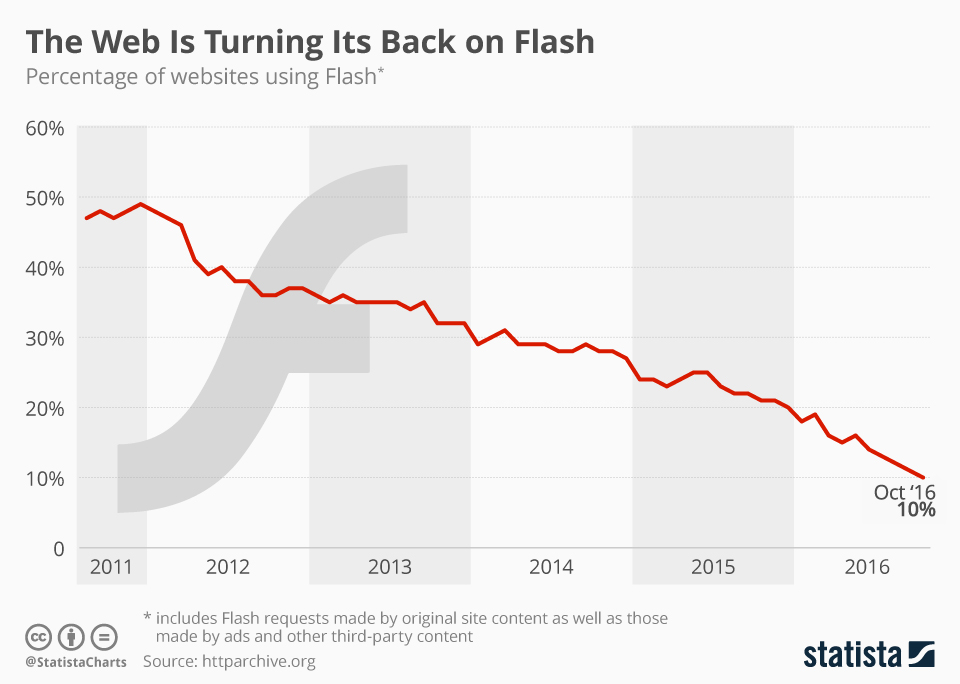
\includegraphics[scale=0.35]{flash-usage}}
\centering
\caption{The decline in Flash usage across the web}
\label{fig:flash-usage}
\end{figure}

\subsection{Font Fingerprinting}

Prevention of font fingerprinting was another important part of the project.
Font fingerprinting through Flash had already been prevented through disabling it altogether, which left the problem of how to stop font fingerprinting through JavaScript.
This was what seemed like an impossible problem, as the browser will use whatever fonts are installed.
After much research, it seemed that there was no method of disabling fonts or concealing them at the add-on level, since it could be altered using CSS, which is too low-level for an add-on to interfere with.

This was a big problem for the project, as font fingerprinting amounts for roughly 7.6 bits of entropy for a sample size of 1,000 users \citep{font-metrics}.
Observing Figure~\ref{fig:font-metrics}, one can see the highest (black) line indicates the maximum entropy if every browser has a unique set of fonts, and the (red) line beneath indicates the entropy available from checking the installed fonts.

\begin{figure}[h!]
\fbox{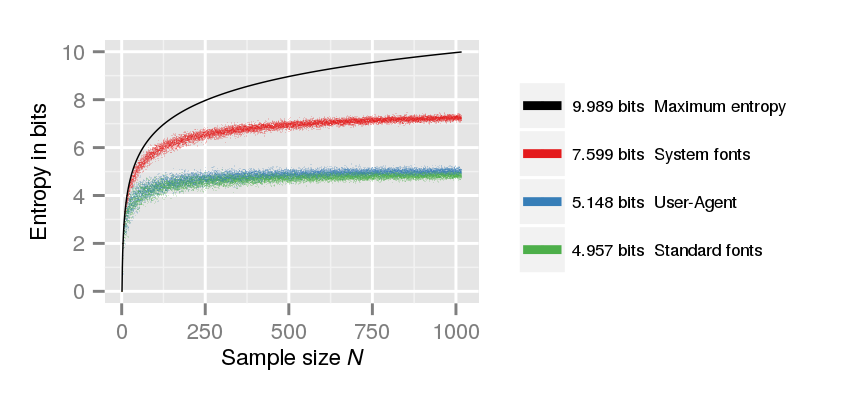
\includegraphics[scale=1.3]{font-metrics}}
\centering
\caption{Graph of entropy vs.\ sample size for font fingerprinting.}
\label{fig:font-metrics}
\end{figure}

Thankfully version 52 of Firefox released on the 7th of March 2017.
In this version of Firefox, a new feature was added that allows users to define a list of `whitelisted' fonts which Firefox will use as if they are the only fonts installed on the system.
This allowed me to change a setting in Firefox's config files, effectively limiting the system fonts to a select few.

\subsection{Prevent Canvas Fingerprinting}

Preventing Canvas fingerprinting was the most difficult part of the project by far.
This is due to a number of problems and roadblocks that materialised during the development of the add-on.
The original plan was for the add-on to simply listen to the webpage for changes once it begins to load, and when the page changes, scan any added nodes for any \texttt{<canvas>} elements, and change the objects themselves to restrict the relevant APIs.
This is essentially what the final product does, though it's not as simple as initially thought.

The main functions that need to be blocked are explained in Table~\ref{tab:canvas-methods}.

\begin{table}[h!]
\centering
\begin{tabular}{| p{6cm} | p{8cm} |}
    \hline
    \textbf{<canvas> function} & \textbf{Description} \\ \hline
    \texttt{context.measureText()} & {Returns the size of text in the canvas element} \\ \hline
    \texttt{context.getImageData()} & {Returns an object containing data about \newline the canvas element inluding a full pixel map} \\ \hline
    \texttt{canvas.toDataUrl()} & {Returns a URL which contains the canvas \newline itself (fully rendered)} \\
    \hline
\end{tabular}
\caption{Table explaining \texttt{<canvas>} functions that need to be restricted}
\label{tab:canvas-methods}
\end{table}

Two of the functions that need to be blocked come from the \texttt{context} object.
The context of a \texttt{canvas} is an object which is used to write to and read from the \texttt{canvas}.
For this reason, blocking access to the context object and to the \texttt{toDataUrl()} function seemed like good first steps to take.
To do this it was clear that a content script (a script that runs locally in every browser tab) was required.
The first objective was to make sure that the add-on could detect \texttt{<canvas>} elements, as it could be built up easily from that initial step.
For this, a JavaScript \texttt{MutationObserver} was used.
This is an object which takes a callback function as a parameter, and then is used to `listen' to a HTML node on a webpage.
Whenever that node changes (or its child nodes), the changes are passed to the callback function.
The first iteration simply prints to the browser console when a \texttt{<canvas>} element is encountered, shown in listing~\ref{lst:canvas-logger}.

\begin{figure}[h!]
\begin{lstlisting}
function onMutation(mutations) {
    for (var i = 0; i < mutations.length; i++) {
        var addedNodes = mutations[i].addedNodes;
        for (var j = 0; j < addedNodes.length; j++) {
            var node = addedNodes[j];
            var found = [];
            if (node.nodeName === 'CANVAS') {
                found.push(node);
            } else if (node.children && node.children.length) {
                found = node.getElementsByTagName('canvas');
            }
            for (var k = 0; k < found.length; k++) {
                console.log("Found a canvas");
            }
        }
    }

}

var observer = new MutationObserver(onMutation);
observer.observe(document, {
    childList: true,
    subtree: true
});
\end{lstlisting}
\caption{A script that listens to a webpage, and prints to the console when a \texttt{<canvas>} element is added}
\label{lst:canvas-logger}
\end{figure}

This worked to a degree, it could not detect canvas elements in within \texttt{<iframe>} HTML elements.
These are elements which load in content from another web page either on the same site or from an external website.
However, this was not realised until later in development.

Once this logging worked, the next step was to try to change the APIs for each of the \texttt{<canvas>} elements on the page.
To do this, instead of simply printing to console when a canvas was added, the JavaScript method \texttt{Object.defineProperties()} was used to change the functions for each element that the script encountered.
To start with, just the \texttt{getContext()} function was blocked, since this prevents writing to and reading from the element.
This didn't work when written in the same way that Figure~\ref{lst:canvas-logger} was written.
The reason behind this is that add-on content scripts have restricted permissions, and can not directly make changes to JavaScript objects defined by the web page, they can only alter the DOM itself.

After discovering this, and researching if it is possible to bypass this security feature, an exploit was discovered.
It works by injecting a \texttt{<script>} node to the beginning of the HTML document that contains the webpage.
This script contains similar code to Figure~\ref{lst:canvas-logger}, though instead of being executed with the permissions clearance of an add-on (unable to change JavaScript objects), it is executed as if it was always part of the web page.
A simple version of this is shown in Figure~\ref{lst:injection}.

\begin{figure}[h!]
\begin{lstlisting}
var actualCode = '(' + function() {
    // Contents of the injected script go in here
} + ')();';

var s = document.createElement('script');
s.textContent = actualCode;
document.documentElement.appendChild(s);
s.remove();
\end{lstlisting}
\caption{Injecting a script into the web page}
\label{lst:injection}
\end{figure}

This method was successfull in breaking \texttt{<canvas>} elements, and meant that they could not be drawn to and data could not be retrieved from them.
However this still did not work for \texttt{<iframe>} elements.
In addition, the script did not prevent \url{browserprint.info}, a website with a fingerprinting test, from acquiring a canvas fingerprint from the browser.

\begin{figure}[!tbp]
    \centering
    \begin{minipage}[b]{0.4\textwidth}
        \fbox{
\includegraphics[width=\textwidth]{hello-world-canvas}}
        \caption{A \texttt{<canvas>} element without the add-on running}
        \label{fig:hello-world-canvas}
    \end{minipage}
    \hfill
    \begin{minipage}[b]{0.4\textwidth}
        \fbox{
\includegraphics[width=\textwidth]{blank-canvas}}
        \caption{The same \texttt{<canvas>} element with the add-on running}
        \label{fig:blank-canvas}
    \end{minipage}
\end{figure}

This problem was difficult to solve, but after sending and receiving an email to and from the team at Browserprint, the solution was much clearer.
The \texttt{<canvas>} element in question does not need to be in the DOM itself to be used to fingerprint, it can be done solely through JavaScript, using the \texttt{document.createElement()} JavaScript function to create a canvas.
This meant that \texttt{createElement()} function needed to be altered for every web page, as well as listening for any actual \texttt{<canvas>} elements added to the page.
Although it is simple enough to prevent access to the function, it is not a satisfactory solution as it is a function that is used to add any HTML nodes to a website, so without it almost all non-static web pages break.
Figure~\ref{lst:create-element} shows how this is achieved without breaking the function entirely.
\texttt{createElement()} takes the name of the HTML element to create as an argument, so when a \texttt{<canvas>} element is desired, one passes \texttt{"canvas"} as an argument to the function.
The function was re-written to check to see what the argument is, and in the case that a canvas is being created, the function will return an \texttt{undefined} object instead of a canvas.

\begin{figure}[h!]
\begin{lstlisting}
document.createElement = function(create) {
    return function() {
        var ret = create.apply(this, arguments);
        if (ret.tagName.toLowerCase() === "canvas") {
            return undefined;
        }
        return ret;
    }
}(document.createElement)
\end{lstlisting}
\caption{The rewriting of the \texttt{createElement() function}}
\label{lst:create-element}
\end{figure}

This successfully prevents canvas fingerprinting on websites in most cases.
One case that this does not solve for as mentioned before is for when there is a canvas within an \texttt{<iframe>}.
This is because the \texttt{MutationObserver} can not access the contents of an iframe that is added to the node that it is monitoring.
For this reason, the app has to find iframes in the same way that it scans for \texttt{<canvas>} elements, but then has to do some processing after it has gathered them.
After acquiring the list of iframes that are added to the page, each one then needs to be scanned in the same way as the entire page was, so another \texttt{MutationObserver} is attached to the iframe, listening for any changes within.
The plan was to do much the same method of breaking certain APIs of the \texttt{<canvas>} elements within the iframe.
This method unfortunately does not work.
If the iframe is loaded in from a different domain than the one that owns the parent webpage, then the parent webpage (and by consequence the script that is injected by the add-on) can not access the contents of the iframe.
This is due to the same-origin policy of web browsers \citep{same-origin}.

The only solution that could be reached at the add-on level was too remove iframes from pages entirely.
Needless to say this is not a usability-friendly solution for mitigating fingerprinting, as iframes are used a great deal on the web.
This was implemented similarly to the method of finding canvas nodes, except instead of merely altering the APIs of the JavaScript objects, then entire object is deleted.
After visiting a few websites it was clear that this was not a very good solution and is not feasible as a long-term method of defence.
\url{panopticlick.eff.org}, another online fingerprint checker can not successfully take a fingerprint when the add-on is activated with the iframe deletion code in effect.
Although it may be seen as a positive thing that a fingerprinter does not work, this is not the case for other comparable fingerprinting websites.
Many other sites simply do not function with the deletion of all of the iframe content on their pages.
This is yet another reason why preventing fingerprinting at the add-on level is difficult.

